\documentclass[a4paper, twoside, 12pt]{report}
\usepackage[
  inner=30mm,
  outer=20mm,
%  textwidth=345pt,
  top=24mm,
  bottom=22mm
]{geometry}

%\usepackage[top=15mm, bottom=22mm]{geometry}
\usepackage{fancyhdr}
\usepackage{framed, color}
\usepackage{graphicx}
\usepackage{url}

\pagestyle{fancy}

\graphicspath{{./images/}}

%% Let's do some macros

\newenvironment{dedication}
  {\clearpage           % we want a new page
   \thispagestyle{empty}% no header and footer
   \vspace*{\stretch{1}}% some space at the top 
   \itshape             % the text is in italics
   \center          % center of the page
  }
  {\par % end the paragraph
   \vspace{\stretch{3}} % space at bottom is three times that at the top
   \clearpage           % finish off the page
}


\makeatletter

\newcommand\frontmatter{%
    \cleardoublepage
  %\@mainmatterfalse
  \pagenumbering{roman}}

\newcommand\mainmatter{%
    \cleardoublepage
 % \@mainmattertrue
  \pagenumbering{arabic}}

\newcommand\backmatter{%
  \if@openright
    \cleardoublepage
  \else
    \clearpage
  \fi
 % \@mainmatterfalse
   }

\makeatother


  
  
\title{\textbf{Entity Relationship Keyword Queries \\ on Knowledge Graph}}
\author{
		\bf{Undergraduate Thesis Report}\\
        \\
        \emph{Submitted in partial fulfilment of requirements for the degree of}\\
        \\
        \bf{Bachelor of Technology (Honours)}\\
        \\
        \emph{by}\\
        \\
		\bf{Pratyaksh Sharma}\\
        \bf{Roll No : 120050019}\\
        \\
        \emph{under the guidance of}\\
        \\
		\bf{Dr. S. Sudarshan}\\
        \\\\
        
\includegraphics[height=3.5cm]{iitb_logo.jpg}\\
        \\
		\bf{Department of Computer Science and Engineering}\\
        \bf{Indian Institute of Technology Bombay}\\
        \bf{Mumbai 400076, India}\\
}
\date{November, 2015}

\bibliographystyle{plain}

\begin{document}
\frontmatter

\maketitle


%%%% Dedications page %%%%
\begin{dedication}
To my parents, for their endless support \\
 without ever having to ask me what I exactly do.
\end{dedication}
%%%% End dedications page %%%%


%%%% Begin acknowledgements page %%%%
\renewcommand{\abstractname}{Acknowledgements}

\begin{abstract}
  I must acknowledge a great debt to my advisor, Professor S. Sudarshan, for his constant advice has been the guiding force throughout and without which, this work would never have been possible. 
  \\ \\
Pratyaksh Sharma
\end{abstract}
%%%% End acknowledgements page %%%%


%%%% Begin abstract page %%%%
\renewcommand{\abstractname}{Abstract}
\begin{abstract}
  The proliferation of structured knowledge bases in recent times and their success in assisting web search has led to a good amount of research dedicated to querying these knowledge bases. While several approaches have been successful at supporting queries of a simple nature, the two main shortcomings of all approaches to querying knowledge bases are: 1) difficulty in formulating queries without familiarity with the knowledge-base schema, and 2) unsatisfactory performance, both in terms of resource (and time) consumption and accuracy of results. In this work, we first survey many of the approaches to various querying problems on structured data. We then present a novel query model and processing framework that will address the deficiencies of existing approaches, in particular, towards supporting complex queries.

\end{abstract}
%%%% End abstract page %%%%


\tableofcontents

\mainmatter


\pagebreak

\chapter{Introduction}

While the web is without doubt the largest collection of human knowledge, it is largely constituted of unstructured information  -- web pages with text, images and other media embedded within them. This organization (or the lack of) of information, poses certain difficulties and inherent limitations in building automated systems that can consume and process information. 

To remedy some of the perceived challenges, there is an ongoing effort to build and maintain structured knowledge bases. As of today, there exist several of such knowledge repositories, for example: Freebase, DBpedia, Wikidata, etc. Apart from those freely accessible, several internet businesses like Google. Yahoo!, and Baidu maintain their own proprietary knowledge bases, which have been used successfully in assisting internet web search applications.

In the wake of increasing popularity structured data and  in order to provide a common platform for data exchange the World Wide Web Consortium decided to collect these efforts under the umbrella of Semantic Web. The Semantic Web is a an extension of the Web through standards  that promote common data formats and exchange protocols on the Web, most fundamentally the Resource Description Framework (RDF).

Even though the attempt is towards giving \emph{structure} to data, the traditional concepts of relational schema and relational data model are eschewed. The data is most commonly modelled as a graph of entities and objects, with an accompanying schema and an ontology. This means that well developed ideas of querying on relational databases can no longer be directly applied; and towards this end query languages such as SPARQL and corresponding query processing engines have emerged.

An important feature of modern knowledge bases is their vastness. Knowledge bases with as many as a billion facts are widely available. While SPARQL and other structured query languages have a number of strong points, their usability is hindered by the limited schema knowledge available to an end user. Therefore, approaches akin to keyword querying in databases, that abstract out schema requirements from the user, have become increasingly relevant.

In this work, we shall survey a number of such keyword querying approaches on structured knowledge bases. We shall also highlight a common weakness in all of them---insufficient performance on complex queries that involve several \emph{joins}. Our own approach towards keyword querying will aim to address this limitation of existing approaches.

\section{Outline}

As a prerequisite to begin our exposition, we provide  an overview of RDF/SPARQL specifications and related concepts in Chapter 2. In Chapter 3, we survey a few select works whose motivation is similar to ours. We highlight important ideas that can be incorporated in building future systems. Finally, Chapter 4 shall provide a detailed discussion of our proposed approach towards the problem. We conclude with the summary and directions for future work in Chapter 5.


\chapter{Background}


In this chapter, we cover the necessary background required for appreciation of this work and the area in general. We begin by describing two of the fundamental building blocks of Semantic Web: 1) Resource Description Format (RDF) that allows a flexible representation of structured information, and 2) the SPARQL query language used to retrieve and manipulate data stored in RDF. Towards the closing, we introduce the Freebase knowledge base---the structured data source that shall be considered primary for the remaining part of this work.


\section[RDF]{Resource Description Format}

Before we dive in head first into the territory of semantic web, we must first understand how it stores data. We start from the ground up by outlining the basic idea of conceptualizing data as a graph---an approach that is many ways contrasted to the relational model assumed by traditional databases.

The fundamental building block of \emph{knowledge graph} (as we shall call it when emphasizing its graph structure), is the notion of an entity. In most applications modelling general-purpose real world information, an entity is something hat has separate and distinct existence and objective or conceptual reality. To make it more concrete, here a few examples of entities:
\begin{itemize}
  \item Indian Institute of Technology, Bombay - an educational institute.
  \item Mumbai - a city
  \item An Evening in Paris - a Bollywood film
  \item Sania Mirza - a person
\end{itemize}

To put it simply, a structured knowledge base captures information about entities. Entities can be related to each other and can have properties (or attributes). The idea of expressing relations between entities is directly borrowed from the notion of Entity-Relationship Model.

Resource Description Framework (RDF) is a framework for representing information about entities in a graph form. It formalizes the notion of entities and relationships between them and the graph thus produced. 

An RDF-triple is a 3-tuple of (subject, predicate, object). While the subject is typically an entity, the object is allowed to be an entity or a non-entity. An RDF object is allowed to be an arbitrary string, which makes it flexible in capturing information such as dates, addresses, and other metadata information that a subject (entity) can be associated with. An RDF predicate is the realization of the concept of a relationship that describes the nature of association between the corresponding subject and object.

\begin{figure}[h!]
  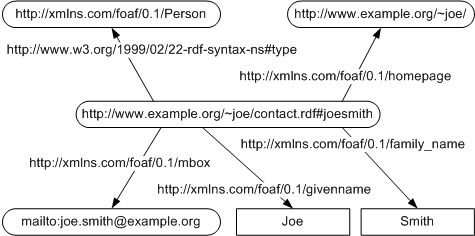
\includegraphics[scale=0.8]{joe-smith-rdf.jpg}
  \caption{An example RDF graph}
  \label{fig:rdfexample}
\end{figure}


Since the RDF evolved around WWW, it encodes the subject, predicate and at times, the object as well, as Uniform Resource Identifiers (URI). An RDF document consists of RDF-triples, typically one triple per line. Figure \ref{fig:rdfexample} illustrates an example RDF graph that the following RDF document represents:

\begin{verbatim}
1: <http://www.example.org/~joe/contact.rdf#joesmith>
      <http://www.w3.org/1999/02/22-rdf-syntax-ns#type>  
      <http://xmlns.com/foaf/0.1/Person>
2: <http://www.example.org/~joe/contact.rdf#joesmith>   
      <http://xmlns.com/foaf/0.1/homepage>
      http://www.example.org/~joe
3: <http://www.example.org/~joe/contact.rdf#joesmith>  
      <http://xmlns.com/foaf/0.1/mbox>
      mailto:joe.smith@example.org
4: <http://www.example.org/~joe/contact.rdf#joesmith>
      <http://xmlns.com/foaf/0.1/givenname>
      Joe
5: <http://www.example.org/~joe/contact.rdf#joesmith>  
      <http://xmlns.com/foaf/0.1/family_name>
      Smith
\end{verbatim}

RDF predicates are represented as labelled arrows that connect an RDF subject (at their tail) to an RDF object (at their head).

Many of the contemporary freely accessible knowledge bases support their distribution in RDF format. While an RDF document is natural way of representing and storing graphs, it is seldom useful in this form. Several RDF databases have emerged that allow loading of RDF documents support APIs that can be used to query and make use of the data. Traditional query languages like SQL are not well suited for querying RDF data, and thus there is a need for query languages and query processing engines that are targeted towards this format. SPARQL is one such query language that has been successful, and we shall now present its brief overview. 


\section[SPARQL]{SPARQL Protocol and RDF Query Language}

SPARQL (recursive acronym for SPARQL Protocol and RDF Query Language) is a semantic query language for RDF databases. SPARQL allows users to write queries against what can loosely be described as ``key-value" data or, more specifically, data that follows the RDF specification of the W3C. 

Though we earlier presented the RDF data model as a graph, it can also be thought of in terms of the SQL relational model as a table with three columns, one each for the subject, the predicate and the object. As we noticed earlier, the data in the object column can be heterogeneous in general, which in contrast with relational databases. The column data type is usually implied by the predicate value or may be specified separately in an ontology. 

As another alternative, all triples belonging to a particular subject may be represented as a single row of the table where the subject is the primary key. A column for each possible predicate may be stored, with the value in a cell storing an RDF object for (row, column) pair of (subject, predicate). However, as is seen in real world datasets, a column could contain multiple values (like the column `family members') for the same row key.

SPARQL provides a full set of analytic query operations such as JOIN, SORT, AGGREGATE for data whose schema is intrinsically part of the data rather than requiring a separate schema definition. Schema information (the ontology) is often provided externally, though, to allow different datasets to be joined in an unambiguous manner. In addition, SPARQL provides specific graph traversal syntax for data that can be thought of as a graph.

\subsection{Example Query}

We shall now illustrate the basic syntax and features of SPARQL using a simple query on the data of Figure \ref{fig:rdfexample}. 

The SPARQL query for retrieving (person, homepage) pairs for all persons in the data, is:
\begin{verbatim}
  PREFIX foaf:   <http://xmlns.com/foaf/0.1/>
  PREFIX w3: <http://www.w3.org/1999/02/22-rdf-syntax-ns>
  FROM foaf:graph
  
  SELECT ?person ?homepage WHERE {
  ?person w3:type foaf:Person,
  ?person foaf:homepage ?homepage
  }
  ORDER BY ?person
\end{verbatim}

Since RDF subjects and predicates are represented as URIs, they tend to have common prefixes. To prevent repetition of these prefixes in the query, the \verb|PERFIX| keyword has been used in the above query. In general, an RDF database might contain multiple RDF graphs. The from keyword allows a user to specify a particular graph to be queried.

The \verb|SELECT| clause asks to specify variables, which are then matched by the triple patterns inside the \verb|WHERE| clause. A triple pattern is simply an RDF triple, whose one or more elements have been replaced by variables. 

It is worth noting that triple patterns allow a natural way of expressing joins without an explicit schema, which makes SPARQL more powerful than storing RDF in a relational schema and running SQL queries on it as was previously discussed.

SPARQL has been implemented in a number of programming languages and graph databases. In particular the Apache Jena Framework and Openlink Virtuoso are widely used implementations of the standard.

\section{The Freebase Knowledge Base}

What was it?

Current status

Idiosyncrasies



\chapter[Survey]{Survey of Existing Work}

This chapter aims to give an overview of the existing work that tackles the problem of querying structured knowledge bases. As we discussed in Chapter 1, the use of structured query languages (e.g. SPARQL) is limited by requirement that the user must be aware of schema of the queried data. We will see in this chapter multiple approaches that seek to remedy that. A full coverage and critique of all approaches is beyond the scope of this report, so we shall select a few interesting ones for the purpose of this chapter. The approaches will be organized by their central ideas.

\section[Keyword Queries]{Free-Keyword Querying}
 
 In \cite{elbassuoni2011keyword}, the authors develop a retrieval model that enables users to search RDF graphs using keywords. In contrast to approaches that retrieve entity tuples, the model here returns a ranked list of RDF \emph{subgraphs}. Retrieving subgraphs allows the treatment of triples in a holistic manner by explicitly taking into account the relationships between entities.
 
 To process keyword queries over RDF graphs, the system associates each triple $t_i$ with a set of keywords derived from the subject and object of the triple, as well as representative keywords for the predicate and constructs a document $D_i$. The terms in the document $D_i$ are stemmed using any standard stemmer and then stored in an inverted index. In addition, the term frequency of term $w$ in $D_i$, referred to as $c(w, D_i)$, is also stored.
 
 The first step towards query processing is to retrieve a set of subgraphs that match the user keyword query. To avoid retrieving large and noisy subgraphs, the following constraints are imposed: 1) the subgraphs should be unique and maximal (no subgraph should be a subset of any other subgraph retrieved), and 2) the subgraphs should contain triples matching different sets of keywords (no triples in the same subgraph should match the exact same set of keywords). The rationale behind the latter constraint is that if two triples match the same set of keywords, they are parts of two different possible results to the user query, and should be considered as parts of two separate subgraphs.
 
 Let the keyword query be $q = \{q_1, q_2, ..., q_m\}$, the subgraph-retrieval algorithm utilizes the inverted index to retrieve lists $\{L_1, L_2, ..., L_m\}$. The set $E$ of all unique triples in all lists can be viewed as a disconnected graph\footnote{each triple can be viewed as an edge where its subject  and object are nodes} and is referred to as the query graph. An adaptation of the network-motif detection algorithm \cite{wernicke2005faster} is used on $E$ to retrieve the desired subgraphs. We omit the discussion here.
 
 On retrieving a set of subgraphs matching a given keyword query, the next step is to rank these subgraphs. The ranking model is based on statistical language model techniques \cite{ponte1998language}. Given a subgraph $G = \{t_1, t_2, ..., t_n\}$, where $t_i$ is a triple, and the query $q = \{q_1, q_2, ..., q_m\}$ where $q_i$ is a single term, the subgraph G  is ranked based on the probability of generating the query Q given the subgraph $G$'s language model. Independence is assumed between the query terms, and likelihood $\text{Pr}(q|G)$ is computed as:
 $$ \text{Pr}(q|G) = \prod_{i=1}^{m} \text{Pr}(q_i|G)$$
 where $\text{Pr}(q_i|G)$ denotes the probability of term $q_i$ in the language model of $G$. The language model of subgraph $G$ is computed as a mixture model of the language models of its constituent triples, 
 
 $$ \text{Pr}(q_i|G) = \frac{1}{n} \sum_{j=1}^{n} \text{Pr}(q_i|t_j)$$

 where $\text{Pr}(q_i | t_j)$ is computed from the document $D_j$ constructed earlier.
 
 The performance of the above model is compared with well-known techniques for keyword search over structured data \cite{bhalotia2002keyword, nie2007web} and we refer the interested reader to the original paper \cite{elbassuoni2011keyword} for that.
 
 
\section{Converting queries to SPARQL}

DEANNA \cite{yahya2012deep} is a framework for natural language question answering over structured knowledge bases. The approach followed by DEANNA is to convert the natural language question to an appropriate SPARQL query that can be then processed over the knowledge base. By far, the main challenge addressed is that of disambiguating user intent expressed in the verbal phrases and noun phrases in the question, and doing this in a globally coherent manner.

As a first step, phrases are detected in the natural language question that potentially correspond to semantic items. This phrase detector unit uses multiple detectors, each of which can detect a certain class of phrases, corresponding to semantic classes, entities, relations and interrogative pronouns. The detectors utilize different named entity recognition and relation detection techniques.

Next, the system attempts to detect \emph{triploids} in the natural language question. A triploid are 3-tuple of tokens which corresponds to a relation and its two arguments. These triploids and the candidate phrases from the previous step are are consolidated into \emph{q-units}, which are phrase-level triples (can possibly have multiple candidates for a relation and arguments).

\begin{figure}
  \center
  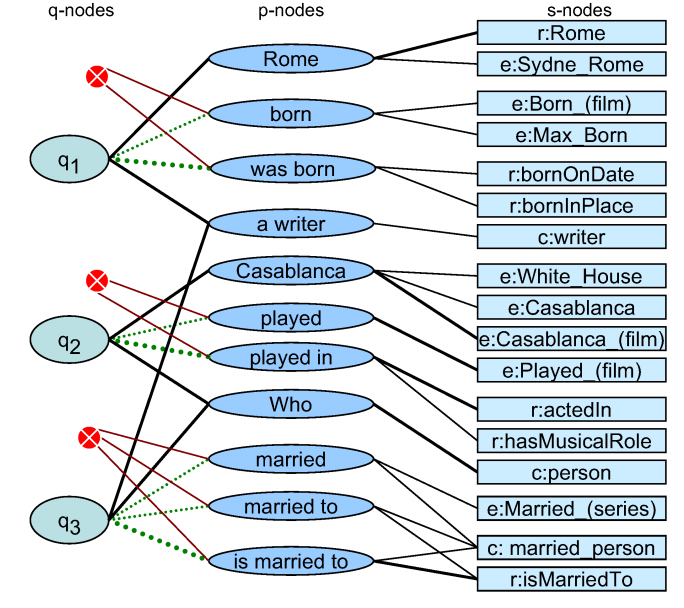
\includegraphics[scale=0.5]{./deanna1.png}
  \label{fig:disgraph}
  \caption{Disambiguation graph. Attribution: \cite{yahya2012deep}}
\end{figure}

The next (and probably the most interesting) step is to perform disambiguation to resolve the mappings of phrases to semantic items. This is done in a joint manner---a weighted disambiguation graph is constructed and a dense subgraph is sought. A disambiguation graph (Figure \ref{fig:disgraph}) is a 3-partite graph with weighted edges. The edge weights are given as a combination of semantic coherence and syntactic similarity. Q-nodes collect triples of phrases together and this can been seen as dotted edges in Figure \ref{fig:disgraph}. 

The problem of disambiguation now translates to finding a dense subgraph in the disambiguation graph. The density measure is a function of edge weights (which measure syntactic similarity and semantic coherence). Further constraints are put on the subgraph such that it represents a valid triple. The objective and the constraints are encoded as an integer linear program and fed into an ILP solver---which then returns the required subgraph.

Once the disambiguation is completed, semantic grouping is performed which forms semantic triples. For example, if it is determined that the relation \texttt{marriedTo} connects the person referred to by `Who' and the \texttt{writer} to form the semantic triple \texttt{person marriedTo writer}. These semantic triples are transformed into SPARQL queries using a rule based method. For example, \texttt{person marriedTo writer} is transformed to \texttt{?x type person}, \texttt{?x marriedTo ?w}, \texttt{?w type writer}.

%---------------GQBE Start----------------------------

\section{Querying by example entity tuples}


 GQBE \cite{jayaram2013querying} proposes to query knowledge graphs by example entity tuples. The user input and output of GQBE are both entity tuples,
called query tuples and answer tuples, respectively. Plainly stated, given a data graph $G$ and a query tuple $t$, GQBE tries to find the top-$k$ answer tuples $t'$ with the highest similarity scores $\text{score}_t(t')$.
 
 
 $\text{score}_t(t')$ is computed by matching the inter-entity relationships of $t$ and that of $t'$. Matching is not done on an entity-level in $t$, rather, a neighborhood graph is constructed (captures `features' that might be of interest to users) from $t$ and $\text{score}_t(t')$ entails matching two
 graphs constructed from $t$ and $t'$ respectively.
 
 The neighborhood graph $H_t$ of an example tuple $t$ is a weakly connected undirected subgraph of $G$ (the data graph) consisting of all nodes reachable from nodes of $t$ by an undirected path of length less than a user defined threshold $d$.
 
 It is observed that $H_t$ can be enormously large even for small values of $d$ (800K nodes for $d = 2$ in case of Freebase). Therefore, GQBE constructs a Maximum Query Graph (MQG) from $H_t$ which is expected to be drastically smaller than $H_t$ and yet capturing important features of the query tuple. $MQG_t$, given
 a parameter $m$, is a weakly connected subgraph of the  neighborhood graph $H_t$ that maximizes total edge weight
 $\sum_e w(e)$ while satisfying the constraints that it contains all the nodes in $t$, and contains at most $m$ edges.
 
 The decision version of finding $MQG_t$ for a given $m$ is shown to be NP-hard, and therefore GQBE employs a greedy algorithm to get an approximate $MQG_t$.
 
 Given a $MQG_t$, the goal is to find answer graphs $A$ which have high similarity to $MQG_t$. An answer graph $A$ to a query graph $Q$ is a
 weakly connected subgraph of $G$ that is edge-isomorphic to $Q$. Similarity is defined as a composite of a content-score and a structure-score. Structure-score captures measures the important structure in $MQG_t$ that is captured by $Q$. Content-score is defined by giving extra credit for identical nodes among the matching nodes in answer graph $A$ and query graph $Q$.
 
 Finally, GQBE searches $G$ for the top-$k$ answer subgraphs (according to the similarity score) in a best-first manner. We omit the algorithm in this discussion. 
 
 \section{Interactive Queries}
 
 Next, we cover FreeQ \cite{demidova2012freeq} - an interactive interface for incremental query construction. It enables a user to start with simple keywords and incrementally refine them into a structured query that captures the user's information need. Figure \ref{fig:freeq} illustrates the FreeQ user interface.

 \begin{figure}[h!]
 %\centering
 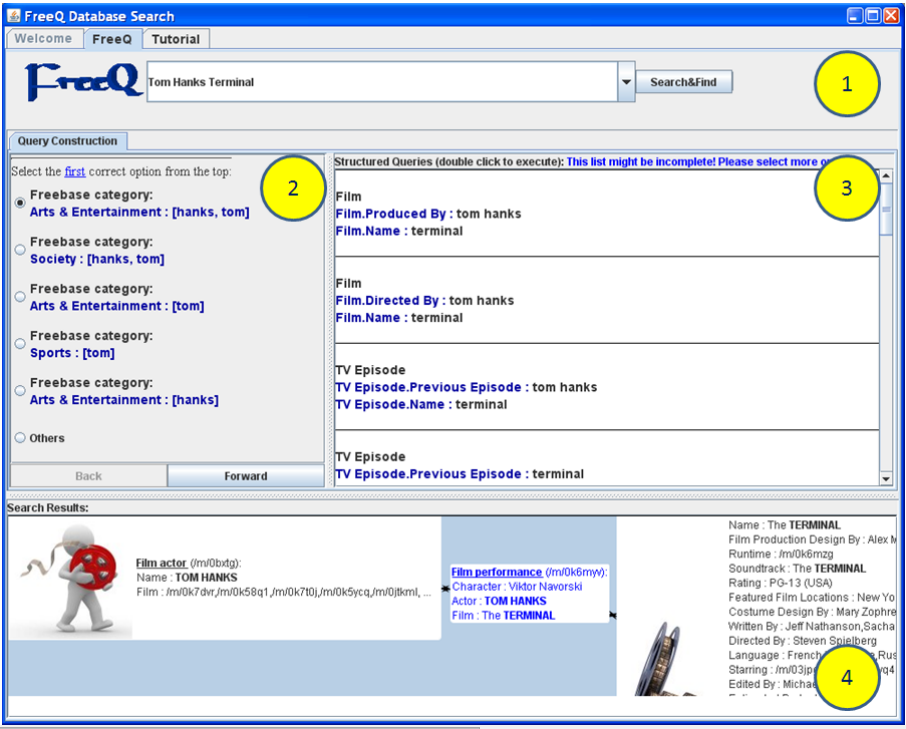
\includegraphics[scale=0.45]{freeq.png}
 \caption{FreeQ GUI. The components of the FreeQ
GUI include: (1) an input field for keyword query,
(2) interaction options, (3) top-k structured queries,
and (4) query results. Attribution: \cite{demidova2012freeq}}
 \label{fig:freeq}
 \end{figure}
 
 When a user issues a keyword query, say \texttt{"Tom Hanks Terminal"}, FreeQ tries to guess the user intent and displays the top-$k$ most likely structured queries in the query window. The user can then click on any of these if it satisfies their information need. 
 
 In the common case, the right structured query will not the identified immediately. The user can then use various interaction options (in the interaction panel) that further clarify intent. These interaction options are simple questions, for example \emph{"Is Tom Hanks a person?"}, and \emph{"Is Terminal an entity in the film domain?"}. Each interaction refines the list of available structured queries to those that comply with the user's selection. 
 
 Conceptually, the main idea is as follows: given a keyword query $K$, the system generates all possible query interpretations of $K$ based on data graph $G$. The set of query interpretations is called the interpretation space of $K$, denoted by $\zeta$. The system also generates a set of interaction options $IO$. If the user selects any interaction option $IO$, the interpretation space $\zeta$ is reduced and further the system displays the top-$k$ interpretations from $\zeta$. The process terminates when the user finds the intended structured query, otherwise it continues generating further interaction options.
 
 It is essential to select the interaction options that can reveal as much information about the user’s intent as possible, i.e., the interaction options with the highest \emph{information gain} need to be identified. FreeQ utilizes the hierarchical conceptual models on top of the database schema to generate interaction options that yield high information gain.
 
 FreeQ extends the Freebase schema with the domain hierarchy of Freebase. Also, FreeQ provides some other types of general interaction options based on hierarchical ontologies. To this end, FreeQ makes use of some external ontologies, such as WordNet \cite{miller1995wordnet} and YAGO \cite{suchanek2007yago}.
 
 The generation of interpretation space is required before top-$k$ interpretations can be obtained. A naive materialization is infeasible for knowledge bases as large as Freebase. FreeQ  uses a query hierarchy introduced in \cite{demidova2012probabilistic}. The hierarchy is grown incrementally during the user interaction phase and generates only the most probable query construction options that comply with the user's selection in each step.
 
 
 
\begin{comment}
\section{Query interpretation based on history}
Fu and Anyanwu [33] propose a context-aware approach for keyword query interpretation that personalizes the interpretation process based on a user’s query context.

In this paper, the problem of generating context-aware query interpretations
for keyword queries on RDF databases by using information from
a user’s query history is addressed. The rationale for this is that users often pose a series of
related queries, particularly in exploratory scenarios. In these scenarios, information
about previous queries can be used to influence the interpretation of a
newer query. For example, given a keyword query “Mississippi River”, if a user
had previously queried about “Mortgage Rates”,then it is more reasonable to
select the interpretation of the current query as being that of a financial institution
“Mississippi River Bank”. On the other hand, if a user’s previous query was
“Fishing Techniques”, it may make more sense to interpret the current query
as referring to a large body of water : the “Mississippi River”. Two main challenges
that arise here include (i) effectively capturing and efficiently representing
query history and (ii) effectively and efficiently exploiting query history during
query interpretation.

The paper proposes and implements a dynamic weighted summary graph model that is
used to concisely capture essential characteristics of a user’s query history.

To achieve this effect, we designed the dynamic weighting function to be
based on a relevance function in terms of two factors: historical impact factor
(hif) and region factor (rf).
Let T indicate the historical index of the most recent query QT , t be the
historical index of an older keyword query Qt, i.e., t $<$ T, and m denote a
summary graph element. Assume that the top-1 interpretation for Qt has already
been generated : QI\textsubscript{t}. Region factor is defined as a monotonically decreasing
function of the graph distance d(m, QIt) between m and QIt:
\begin{align}
rf(d(m, QI\textsubscript{t})) = \frac{1} {a^{d(m,QI\textsubscript{t})}}
\end{align}
Here, a $>$ 1 is a positive integer constant.

Historical impact factor captures the
property that the relevance between a query and a graph element will decrease
when that query ages out of the query history. hif is a monotonically decreasing
function: 
\begin{align}
hif(t) = \frac{1}{b^{T-t}}
\end{align}
where b $>$ 1 is also a positive integer constant.

 
\section{Alternate query languages}
Pound et al. [30] approach the keyword disambiguation problem by ranking different possible rewritings of a query based on their syntactic relationship to the keywords in the query as well as their semantic coherence in the underlying knowledge base. 

In case of unstructured data,
data can be of any type, not necessarily follow any format or rule. e.g. text,video,sound etc. On the other
hand, in case of structured data, the data is organized in semantic chunks(entities). Similar entities are
grouped together to form relations or classes. i.e. in case of structured data, some schema information is
available. As an example ExDB,YAGO have schema items numbering in the millions. So, given such huge
schema information, writing a structured query is a very hard task. This is called Information Overload
Problem. As a naive approach to the above problem, one can use keyword search. But, this comes at a loss of expressivity.
i.e. users can not express desired structure in the query and can not take advantage of schema
information. But, it is very flexible, in the sense that a user can query even if he has no knowledge of the
underlying schema information. On the other hand, conventional structured query is expressive but lacks
flexibility. So, the authors propose a new approach that combines flexibility of keywords as well as expressivity
of structured query, to provide a new query language, called keyword-based structured query
language. e.g. say the information need is “find all people of German nationality who have won a Nobel
award”. Then, the structured query would be
“q(x):- GERMAN PEOPLE(x), hasWonPrize(x, y), NOBEL PRIZE(y)”. The keyword query would be “german
has won nobel award”, and the keyword basedstructured
query would be “german, has won(nobel award)”.


A user enters keyword-based structured query Q to the system. Each keyword k in Q is matched to a set
of schema items using some syntactic similarity measure, with the help of the KB. Each such set forms a
partition. Now, a disambiguation graph G is generated from these. Any induced subgraph of G, that spans
all the partitions, corresponds to a concept query interpretation of Q. Now, these interpretations are ranked
based on some score function that combines semantic and syntactic similarities with the original query Q,
given the KB. Next, top k of those structured queries are evaluated to find potentially relevant entities
and their corresponding documents. The documents are then returned to the user ranked by some relevance
metric.

MashQL [31] present a query formulation language in order to easily query and fuse structured 
data on the web where users can specify filters. It is designed without loss of generality and 
can be used for querying relational databases, XML, RDF and web tables. 

\section{Corpus}
35 propose two new, natural formulations for joint query interpretation and response ranking that exploit bidirectional flow of information between the knowledge base and the corpus.

Here  we  focus  on  a  specific  kind  of  entity  search  query:
Some words (called
selectors
) in the query are meant to occur literally in a response document (as in traditional text
search),  but other words
hint at the type of entity sought
by the query.  Unlike prior work on translating well-formed
sentences or questions to structured queries using deep NLP,
we are interested in handling "telegraphic" queries that are typically sent to search engines.  Each response entity must
be a member of the hinted type.
Note that this problem is quite different from finding answers  to  well-formed  natural  language questions (e.g., in
Wolfram Alpha) from structured knowledge bases (perhaps
curated through information extraction). Also observe that
we do not restrict ourselves to queries that seek entities by
attribute  values  or  attributes  of  a  given  entity  (both  are
valuable query templates for e-commerce and have been re-
searched).   In  our  setup,  some  responses  may  only  be  collected from diverse, open-domain, free-format text sources.
E.g., typical driving
time
between Paris and Nice (the target
type is time duration), or
cricketers
who scored centuries at
Lords (the target type is cricketers).
The  target  type  (or  a  more  general  supertype,  such  as
sportsperson
in place of
cricketer
) may be instantiated in a
catalog
, but the typical user has no knowledge of the catalog
or  its  schema.   Large  catalogs  like  Wikipedia or Freebase
evolve "organically".  They are not designed by linguists, and
they are not minimal or canonical in any sense.  Types have
overlaps  and  redundancies.   The  query  interpreter  should
take advantage of specialized types whenever available, but
otherwise gracefully back o to broader types.


----------------------------
36
We  present  a  new  architecture  for  structural  interpretation of a telegraphic query into these segments:

Mention/s
\^{e\textsubscript{1}}
of an entity
e\textsubscript{1}
,
•
Mention
\^{r}
of a relation type
r
,
•
Mention
\^{t\textsubscript{2}}
of a target type
t\textsubscript{2}
, and
•
Other  contextual  matching  words
s
(some-
times called
selectors
),
with the intent of finding and ranking entities
e\textsubscript{2} $ \in $
t\textsubscript{2}
,  such that
r
(e\textsubscript{1}
, e\textsubscript{2})
is likely
to hold.
Given  the  short,  telegraphic  query  utterances,
we limit our scope to at most one relation mention,
unlike  the  complex  mapping  of  clauses  in  well-
formed  questions  to  twig  and  join  style  queries
(e.g., “find an actor whose spouse was an Italian
bookwriter”). We  present  a  novel  discriminative  graphical
model to capture the entity ranking inference task.

The following notations are used:
\begin{itemize}


\item
$ \Psi $\textsubscript{R}
(q,z,r)
denotes   the   compatibility   be-
tween  the  relation  hint  segment
\^{r} (q,z)
and
a proposed relation type
r
in the KG.
\item 
$ \Psi $\textsubscript{T\textsubscript{2}}
(
q,z,t\textsubscript{2}
)
denotes  the  compatibility  between  the  type  hint  segment
\^{t\textsubscript{2}}
(
q,z
)
and  a
proposed  target  entity  type
t\textsubscript{2}
in  the KG.
\item
$ \Psi $\textsubscript{
E\textsubscript{1}
,R,E\textsubscript{2}
,S}
(
q,z,e\textsubscript{1}
,r,e\textsubscript{2}
)
is a novel corpus-
based evidence potential that measures how
strongly
e\textsubscript{1}
and
e\textsubscript{2}
appear in corpus snippets
in the proximity of words in
\^{s}
(
q,z
)
, and apparently related by relation type
r.
\item
$ \Psi $\textsubscript{
E\textsubscript{1}}
(
q,z,e\textsubscript{1}
)
denotes  the  compatibility  be-
tween the query segment

\^{e\textsubscript{1}}
(
q,z
)
and entity
e\textsubscript{1}
that it purportedly mentions.
\item
$ \Psi $\textsubscript{
S}
(
q,z
)
denotes selector compatibility.  Selectors are a fallback label, so this is pinned
arbitrarily to 1; other potentials are balanced
against this base value.
\item
$ \Psi $
\textsubscript{E\textsubscript{1}
,R,E\textsubscript{2}}
(
e\textsubscript{1}
,r,e\textsubscript{2}
)
is
A
if   the   relation
r
(
e\textsubscript{1}
,e\textsubscript{2}
)
exists in the KG, and is
B $>$
0
otherwise, for tuned/learnt constants
A $>$ B $>$ 0
. Note that this is a soft constraint (
B $>$
0
);
if the KG is incomplete, the corpus may be
able to supplement the required information.
\item
$ \Psi $\textsubscript{
E\textsubscript{2}
,T\textsubscript{2}}
(
e\textsubscript{2}
,t\textsubscript{2}
)
is  1  if
e\textsubscript{2}
belongs  to
t\textsubscript{2}
and
zero otherwise. In other words, candidate
e\textsubscript{2}s
must be proposed to be instances of the proposed
t\textsubscript{2}
— this is a hard constraint, but can
be softened if desired, like
$ \Psi $\textsubscript{E\textsubscript{1},R,E\textsubscript{2}}
\end{itemize}

We perform a MAP inference over all other hidden
variables and note the score of
e\textsubscript{2}
as the product of
the above potentials maximized over choices of all
other variables.\\
score(e\textsubscript{2}) = \\
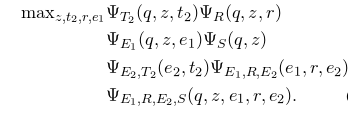
\includegraphics[height=3.5cm]{./1.png}


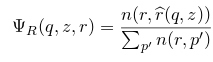
\includegraphics[height=1.5cm]{./2.png}
where
p'
ranges over all phrases that are known to
hint at
r
, and
n
(
r,p
)
denotes the number of sentences where the phrase
p
occurred in the dependency path between the entities participating in relation
r
.

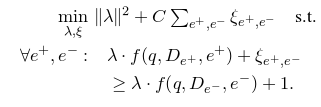
\includegraphics[height=2.8cm]{./3.png}\\
where
e\textsuperscript{+}
and
e\textsuperscript{-}
are positive and negative entities for the query
q
and
f
(
q,D\textsubscript{e}
,e
)
represents the
feature map for the set of snippets
D\textsubscript{e}
belonging
to entity
e
.  The assumption here is that all snip-
pets containing
e\textsuperscript{+}
are “positive” snippets for the
query.
f
consolidates various signals like the number of snippets where
e
occurs near query entity
e\textsubscript{1}
and a relation phrase, or the number of snippets
with high proportion of query IDF, hinting that
e
is a positive entity for the given query.\\

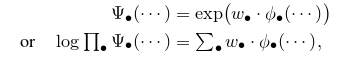
\includegraphics[height=1.8cm]{./4.png}\\

with
w\textsubscript{.}
being a weight vector for a specific potential ., and $ \phi $\textsubscript{.}
being a corresponding feature vector.
During inference, we seek to maximize\\

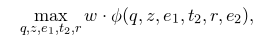
\includegraphics[height=1.5cm]{./5.png}\\

for a fixed
w
, to find the score of each candidate
entity
e
2
.  Here all
w
•
and
φ
•
have been collected
into unified weight and feature vectors
w,φ
. Dur-
ing training of
w
, we are given pairs of correct and
incorrect answer entities
e
+
2
,e
−
2
,  and we wish to
satisfy constraints of the form \\

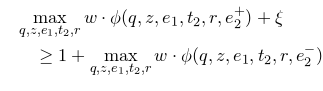
\includegraphics[height=2.3cm]{./6.png}


37
We
propose a structured query mechanism,
entity-relationship
query
, for searching entities in Wikipedia corpus by their
properties and inter-relationships.


\end{comment}

\chapter[ER Keyword Querying]{Entity Relationship Keyword Queries}

% TODO complete outline
In this chapter, we present a detail discussion of our approach towards supporting keyword queries and the techniques used. 

\section{Query Model}

The notion of Entity Relationship Query (ERQ) or Shallow Semantic Query (SSQ) is defined by \cite{li2010structured, li2012entity} as a powerful and flexible query form which allows users to specify expected entity types or categories along with selection predicates for entities and relation predicates for relationship between entities.

For example, a query described as ``Find PERSON \emph{near} \underline{`Stanford graduate'}, and COMPANY \emph{near} \underline{`Silicon Valley'}, where PERSON \underline{founded} COMPANY" can be described in ERQ form as in Figure \ref{fig:erq}.

\begin{figure}[h!]
\centering
\begin{BVerbatim}
SELECT x, y
FROM PERSON x, COMPANY y
WHERE x:['Stanford', 'graduate']
WHERE y:["Silicon Valley"]
AND x,y:['found']
\end{BVerbatim}
\caption{An example ER Query}
\label{fig:erq}
\end{figure}

The query of Figure \ref{fig:erq} seeks the entity pairs \texttt{(x, y)} such that entity \texttt{x} is of type \texttt{PERSON} (and further a Stanford graduate), entity \texttt{y} is of type \texttt{COMPANY} (in particular, a Silicon Valley company) and \texttt{x} has founded \texttt{y}. \texttt{x} and \texttt{y} are entity variables that will bind to entities in the query result. \texttt{PERSON} and \texttt{COMPANY} describe the category/types of these entities. \texttt{"Stanford graduate"} and \texttt{"Silicon Valley"} play the role of selector keywords for entities \texttt{x} and \texttt{y} respectively. Finally, \texttt{found} is the relation keyword describing the relationship between entities \texttt{x} and \texttt{y}.

To make our discussion convenient, we formalize the notion of ERQ as follows. Our system expects the user to specify:

\begin{itemize}
\item The number of entities ($n$) desired in a result. The entity variables will be referred to as $x_1, x_2, ..., x_n$.
\item A list of category keywords $C_i$ for each entity variable $x_i$.
\item A list of \emph{selector keywords} $K_i$ for each entity variable $x_i$.
\item A list of relation keywords $R_{ij}$ describing the relationship between entities $x_i$ and $x_j$ for all $i \neq j$.
\end{itemize}

The result of the query shall be one or more $n$-tuples, where $n$ is as specified in the query. In particular, the elements of the tuple bind to entity variables $(x_1, x_2, ..., x_n)$.

The category keywords are used to specify what category or type the corresponding entity falls in. Selector keywords desire that the corresponding entity be \emph{associated} with these words. Relation keywords specify the relation predicates, in the same manner as ERQ. It is worth noting that each of $C_i$, $K_i$, and $R_{ij}$ may be left empty (unspecified) by the user. The user is also not expected to specify these query keywords in conformity with the schema of the queried RDF graph.

We now illustrate another example to ease understanding of our ERQ formalism. Suppose we want to find the parent-child pairs of US presidents who have attended the same university. Such a query is demanding three entities $x_1$, $x_2$, and $x_3$---$x_1, x_2$ are the presidents, and $x_3$ their common alma mater. A user may formulate the query in the following manner:

\begin{itemize}
\item Number of entities is 3.
\item $C_1=$\{`person'\}, $C_2=$\{`person'\}, and $C_3=$\{`university'\}.
\item $K_1=$\{`US', `President'\}, $K_2=$\{`US', 'President'\}, and $K_3=$\{\}.
\item $R_{12}=$\{`parent'\}, $R_{13}=$\{`education'\}, and $R_{23}=$\{`education'\}, 
\end{itemize}

As we observed in Chapter 3, the problem of segmenting a user keyword query into the keywords for type/categories of entities sought and those for describing relationship between these entities inherently limits the performance (in both precision and recall) of the querying system. The ER query model might seem like a convenient ignorance of such issues, and in many ways it is. Our stance is that ER queries do not expect the amount of user sophistication that SPARQL querying systems expect. It is a sweet compromise between SPARQL querying and free-keyword querying that allows us to focus on challenges beyond query segmentation. Further, we believe that our ideas in this work can be supplemented with a layer of query segmentation---enabling free-keyword querying. 

\section{Query Processing}

The central goal of our work is to enable users to query structured knowledge bases without expecting \emph{any} schema knowledge whatsoever. In the context of the ER query model described previously, this means that keywords supplied in a user query will not in general match those used for data representation in the underlying data source. For example, a user might use the relation keyword \texttt{"established"} to mean ``establishment" of a company or an organization; but in the data source, the actual predicate sought could be \texttt{"founded"}---which roughly means the same as \texttt{"established"} in case of companies. 

Therefore, to achieve superior recall, we must explore many possible \emph{meanings} of a keyword used by the user. 

Further, a user specified keyword could be ambiguous, in the sense that it could could mean any of a number of entities/predicates in the data. To achieve superior precision, we must be able to disambiguate the intent of the user query. 

Our approach towards the above two problems is of asking the user for help. More concretely, our query processing engine shall prompt the user to select a subset of intermediate \emph{candidate} that entities or predicates that the system might be evaluating during query processing. 

Overall, the query processing proceeds with the repeated execution of two steps: 1) Predicate Selection, and 2) Entity Selection.

\subsection{Predicate selection}

As we assume that the user has no familiarity with representation of the underlying data, the relation keywords $R_{ij}$ specified by the user can not, in general, identify a unique predicate in the RDF graph. Therefore, in this stage, the system presents a set of candidate predicates that match the given relation keywords $R_{ij}$. The user is then expected to select of subset of these predicates that align with her intent. It is to be ensured that a small enough, yet accurate enough set of candidate predicates is presented to the user, in order to minimize user effort. This step, referred to as predicate selection for $p_{ij}$, is performed for each of the relations $x_i \sim x_j$ specified initially by the user.

\subsection{Entity selection}

After the user has selected desired set of predicates $\{p^1_{ij}, p^2_{ij}, ..., p^r_{ij}\}$ that comply with the given relation keywords $R_{ij}$, the system shall try to determine the entities $x_i$ and $x_j$ obeying any of these relations.

The RDF graph is queried to find all entities $x_i$ and $x_j$ that match the triple pattern $\langle ?x_i, p^k_{ij}, ?x_j \rangle$ ($k = 1,...,r)$. By the sets $X_i$ and $X_j$, we mean the set of candidate entities thus obtained for entity variables $x_i$ and $x_j$, respectively. These sets $X_i$ and $X_j$ are further filtered, based on the category keywords $C_i$, $C_j$, and selector keywords $K_i$, $K_j$. The resulting sets $\tilde{X_i}$ and $\tilde{X_j}$ obtained after filtering are presented as candidate entities for entity variables $x_i$ and $x_j$.

At this step, the user is expected to select a subset of these entities that align with her intent. As in the case of predicate selection, it is to be ensured that a small enough, yet accurate set of candidate entities is presented to the user. The entity selection step for entity variables $x_i$ and $x_j$ is performed after the predicate selection step for $p_{ij}$.

Once the user agrees on a set of candidate entities $\tilde{X_i}$ for entity variable $x_i$, this information will be used to reduce the complexity of the further entity selection stages. This process terminates when predicate selection and entity selection has been performed for each predicate and entity in the query. The entity-relation graphs are finally ranked and returned to the user as query results.

\subsection{An Example}


\section{Query Interpretation}
Even when we depend on the user's input for disambiguation of the query, we cannot simply blurt out a large set of candidate entities/predicates, for might the user be overwhelmed. Thus, we face the problem of giving an intermediate ranking to candidate entities/predicates, which can then be used to lower down the size of candidate set exposed to the user (in a top-k fashion).

\subsection{Predicate Selection}
A naive approach to populate the set of candidate predicates, would be to scan all possible predicates and discard those whose \emph{descriptions} do not match with the specified relation keywords $R_{ij}$. It is also possible to create a full text index on the predicate descriptions and to query it using $R_{ij}$. As can be expected, this approach is too simple and yields a large set of candidate predicates.

The choice of candidate predicates $p_{ij}$ can be improved by using the category keywords $C_i, C_j$ and the selector keywords $K_i, K_j$ for the entity variables $x_i$ and $x_j$ that are related by $p_{ij}$. Following the success of generative models in entity search \cite{sawant2013learning}, we propose a generative language model for joint query interpretation for choosing candidate predicates.

Let $\vec{q} = (R_{ij}, C_i, C_j, K_i, K_j)$ denote the part of the query pertaining to the predicate $p_{ij}$ and entities $x_i$, $x_j$. We are interested in $\argmax_{p}$Pr$(p|\vec{q})$, where
\begin{align}\label{eq:1}
\text{Pr}(p|\vec{q}) &\propto \text{Pr}(p, \vec{q}) = \text{Pr}(p)\cdot \text{Pr}(\vec{q}|p) = \text{Pr}(p)\cdot \sum_{t_{i}, t_{j}} \text{Pr}(\vec{q}, t_i, t_j | p) \\
&= \text{Pr}(p)\cdot \sum_{t_{i}, t_{j}} \text{Pr}(R_{ij}, C_i, C_j, K_i, K_j, t_i, t_j| p) \\
&= \text{Pr}(p)\cdot \sum_{t_{i}, t_{j}} \text{Pr}(R_{ij}|p)\cdot\underbrace{\text{Pr}(t_i,t_j|R_{ij},p)}_\text{(I)}\cdot\underbrace{\text{Pr}(C_i,C_j|t_i,t_j,R_{ij},p)}_\text{(II)}\cdot \phi_1 \label{eq:omphi1}
%&= \text{Pr}(p)\sum_{t_i, t_j, e_i, e_j} \text{Pr}(R_{ij}|p)\text{Pr}(t_i,t_j|R_{ij},p)\text{Pr}(e_i, e_j|t_i, t_j, R_{ij}, p) \text{Pr}(C_i,C_j|e_i,e_j,t_i,t_j,R_{ij},p)
\end{align}
where $\phi_1$ is defined as:
\begin{align}
\phi_1(K_i,K_j,C_i,C_j,e_i,e_j,t_i,t_j,R_{ij},p) = \text{Pr}(K_i,K_j|C_i,C_j,e_i,e_j,t_i,t_j,R_{ij},p) \label{eq:phi1}
\end{align}
Latent variables $t_i, t_j$ are introduced in (\ref{eq:1}), representing the types of the entities $x_i$ and $x_j$ respectively. The expressions (I) and (II) can be simplified, using the following reasonable independence assumptions:

\begin{enumerate}
\item $\text{Pr}(t_i,t_j|R_{ij},p) = \text{Pr}(t_i,t_j|p)$, i.e., the relation keywords $R_{ij}$ do not convey any extra information when the predicate $p$ is known.

\item $\text{Pr}(C_i,C_j|t_i,t_j,R_{ij},p) = \text{Pr}(C_i,C_j|t_i,t_j)$, i.e., the category keywords are independent of $R_{ij}$ and $p$, once $t_i$ and $t_j$ are known.

\item $\text{Pr}(C_i,C_j|t_i,t_j) = \text{Pr}(C_i|t_i) \cdot \text{Pr}(C_j|t_j)$, i.e., $C_i$ and $C_j$ are independent of each other and of any types other than $t_i$ and $t_j$, respectively.  
\end{enumerate}

Thus, we now have:
\begin{align}
\text{Pr}(p|\vec{q}) &\propto \text{Pr}(p)\cdot \sum_{t_{i}, t_{j}} \text{Pr}(R_{ij}|p)\cdot \text{Pr}(t_i,t_j|p) \cdot \text{Pr}(C_i|t_i) \cdot \text{Pr}(C_j|t_j) \cdot \underbrace{\phi_1}_\text{(III)} \label{eq:main2}
\end{align}

Furthermore, by introducing the latent variables $e_i$ and $e_j$ for entities represented by $x_i$ and $x_j$ in the query, we can rewrite $\phi_1$ as:
\begin{align}
\phi_1 = \text{Pr}(K_i,K_j|&C_i,C_j,t_i, t_j,R_{ij},p) = \sum_{e_i,e_j}\text{Pr}(K_i,K_j,e_i,e_j|C_i,C_j,t_i,t_j,R_{ij},p) \\
&= \sum_{e_i,e_j} \underbrace{\text{Pr}(e_i,e_j|C_i,C_j,t_i,t_j,R_{ij},p)}_\text{(IV)} \cdot \underbrace{\text{Pr}(K_i,K_j|e_i,e_j,C_i,C_j,t_i,t_j,R_{ij},p)}_\text{(V)} \label{eq:ugly2}
\end{align}

Similarly as before, we need the following independence assumptions to simplify (IV) and (V),
\begin{enumerate}
\item $\text{Pr}(e_i,e_j|C_i,C_j,t_i,t_j,R_{ij},p) = \text{Pr}(e_j,e_j|t_i,t_j,p)$, i.e, the category keywords $C_i,C_j$, and the relation keywords $R_{ij}$ do not convey any extra information when the types $t_i,t_j$, and the predicate $p$ is known.

\item $\text{Pr}(K_i,K_j|e_i,e_j,C_i,C_j,t_i,t_j,R_{ij},p) = \text{Pr}(K_i,K_j|e_i,e_j)$, i.e., the selector keywords $K_i,K_j$ are independent of category keywords $C_i,C_j$, the types $t_i,t_j$, the relation keywords $R_{ij}$, and the predicate $p$, once the actual entities $e_i,e_j$ are known.

\item $\text{Pr}(K_i,K_j|e_i,e_j) = \text{Pr}(K_i|e_i)\cdot \text{Pr}(K_j|e_j)$, i.e., $K_i$ and $K_j$ are independent of each other and of any entities other than $e_i$ and $e_j$, respectively.
\end{enumerate}

Therefore, (\ref{eq:ugly2}) reduces to $\sum_{e_i,e_j} \text{Pr}(e_i,e_j|t_i,t_j,p) \cdot \text{Pr}(K_i|e_i) \cdot \text{Pr}(K_j|e_j)$ and (\ref{eq:main2}) now becomes:

\begin{align}
\text{Pr}(p|\vec{q})& \propto \text{Pr}(p) \cdot \sum_{t_i,t_j,e_i,e_j} \phi_2(p, R_{ij}, C_i, C_j, K_i, K_j, t_i, t_j, e_i, e_j) \label{eq:main3}
\end{align}
where $\phi_2$ is defined as,
\begin{align}
\phi_2 = \text{Pr}(R_{ij}|p) \cdot \text{Pr}(t_i,t_j|p) \cdot \text{Pr}(C_i|t_i) \cdot \text{Pr}(C_j|t_j) \cdot \text{Pr}(e_i,e_j|t_i,t_j,p) \cdot \text{Pr}(K_i|e_i) \cdot \text{Pr}(K_j|e_j) \label{eq:phi2}
\end{align}
Arguments to functions $\phi_1$ and $\phi_2$ are omitted in Equations \ref{eq:omphi1}, \ref{eq:main2}, \ref{eq:ugly2} and \ref{eq:phi2}  for the lack of horizontal space.

Throughout this section we have dealt with probabilities and have ultimately arrived at a set of probabilities to be computed. We understand that such probabilities in the Bayesian sense of the word are hard to estimate, if at all well defined. We therefore, tweak our notation a little, replacing probabilities $\text{Pr}$ with potentials $\psi$. The entire derivation continues to hold, even with the modified semantics. 

For the rest of this chapter, we use the following notation:
\begin{enumerate}
  \item $\psi(p)$ in place of $\text{Pr}(p)$: represents the prior weight on the predicate $p$
  \item $\psi(R_{ij}, p)$ in place of $\text{Pr}(R_{ij}|p)$: represents the \emph{compatibility} of keywords $R_{ij}$ and predicate $p$
  \item $\psi(C_i, t_i)$ in place of $\text{Pr}(C_i|t_i)$: represents the \emph{compatibility} of keywords $C_i$ and a Freebase type $t_i$
  \item $\psi(K_i, e_i)$ in place of $\text{Pr}(K_i|e_i)$: represents the \emph{compatibility} of keywords $K_i$ and the Freebase entity $e_i$
  \item $\psi(t_i, p, t_j)$ in place of $\text{Pr}(t_i, t_j|p)$: represents the \emph{compatibility} of the predicate $p$ with the Freebase types $t_i$ and $t_j$
  \item $\psi(e_i, e_j, t_i, t_j, p)$ in place of $\text{Pr}(e_i, e_j | t_i, t_j, p)$: represents the \emph{compatibility} of Freebase entities $e_i$ and $e_j$ with Freebase types $t_i$ and $t_j$ respectively, and of the entities with the Freebase predicate $p$
\end{enumerate}

The potentials $\psi$ used above can be compactly represented as an undirected probabilistic graphical model. We omit the discussion towards this direction for brevity and proceed straight to describing how the above quantities will be estimated.

\subsubsection{Estimating $\psi(p)$}
$\psi(p)$ is simply the prior on the predicate $p$. We estimate it as:
$$\psi(p) = \frac{\text{freq}(p)}{\sum_{p_i \in \mathbb{P}}\text{freq}(p_i)}$$
where $\mathbb{P}$ is the set of all possible predicates in our RDF data source. 

\subsubsection{Estimating $\psi(R_{ij}, p)$, $\psi(C_i, t_i)$, and $\psi(K_i, e_i)$}
The  potentials $\psi(R_{ij}, p)$, $\psi(C_i, t_i)$, and $\psi(K_i, e_i)$ are similar in the sense that they all capture the agreement between two variables: one of them being keywords supplied in the user query and the other being a predicate, type, or an entity in the structured data source. 
For example, if the the relation keywords $R_{ij}$ are \texttt{"death reason"} and the related entity sought is of type \texttt{person}, then $R_{ij}$ should match to the 
predicate \texttt{/people/} \texttt{deceased\_person/} \texttt{cause\_of\_death} rather than the predicate \texttt{/people/} \texttt{deceased\_person/} \texttt{place\_of\_death}.

There may exist considerable variation in how keywords are represented in a query. The relation language model needs to build a bridge between the formal $p$ and the textual $R_{ij}$, so that (un)likely $p$'s have (small) large potential. Plenty of approaches \cite{berant2013semantic, berant2014semantic, kwiatkowski2013scaling, yih2014semantic} to this problem have been studied recently. We choose a pattern-based approach akin to PATTY \cite{nakashole2012patty} for its simplicity and scalability to large amounts of data.

For each Freebase predicate $p$, we discover the most strongly associated phrase patterns from a reference corpus, then mark these patterns into much larger payload corpus. 
The ClueWeb09 corpus annotated with Freebase entities \cite{gabrilovich2013facc1} may be used for this purpose. For each Freebase predicate $p$, we consider all triples and locate all the corpus sentences that mention both the participating entities of the triple. We assume, rather crudely, that if the entities $e_i$ and $e_j$ co-occur in a sentence then this sentence is an evidence of the triple $\langle e_i, p, e_j \rangle$. Each such sentence is parsed to obtain a dependency graph using the Malt Parser \cite{nivre2007maltparser}

We present the approach towards estimating $\psi(R_{ij}, p)$; those for $\psi(C_i, t_i)$ and $\psi(K_i, e_i)$ will be similar and shall be added in later versions of this work. The following brief description is based on \cite{joshiknowledge}.

Words in the path connecting the entities are joined together and added to a candidate phrase dictionary, provided the path is at most k-hops (k is chosen experimentally, we expect that longer dependency paths arise out of noisy sentences/parsing). Thus, we have, for all predicates $p$, a list $\mathbb{R}_{ij}$ of all phrases that are known to hint at $p$. We can then estimate $\psi(R_{ij}, p)$ as:
\begin{align}
\psi(R_{ij}, p) = \frac{n(p, R_{ij})}{\sum_{R'_{ij} \in \mathbb{R}_{ij}}{n(p, R'_{ij})}}
\end{align}
 where $n(p, R_{ij})$ represents the number of sentences in which $R_{ij}$ occurred as a phrase in the dependency path between entities participating in relation specified by predicate $p$.

\subsubsection{Estimating $\psi(t_i,t_j,p)$}
As the potential does not involve any query keywords, it is relatively straightforward to estimate. For the predicate $p$, we identify all the triples that it is involved in, and filter those out  in which the connected subject and object have types $t_i$ and $t_j$ respectively. Let $n(p; t_i, t_j)$ be the number of such triples. Then, simply

\begin{align}
\psi(t_i,t_j,p) = \frac{n(p; t_i, t_j)}{n(p)}
\end{align}
where $n(p)$ denotes the number of triples in Freebase that have $p$ as the predicate.

Note that the filtering operation above can be easily carried out in case of Freebase due to the availability of a \texttt{/object/type/} relation for most entities.

\subsubsection{Estimating $\psi(e_i,e_j,t_i,t_j,p)$}
Though $\psi(e_i,e_j,t_i,t_j,p)$ must take into account the $e_i$--$t_i$, and $e_j$--$t_j$ compatibility, we make a simplifying assumption without deviating a lot from the intended semantics of $\psi(e_i,e_j,t_i,t_j,p)$.

Define, 
\begin{align}
\psi(e_i,e_j,t_i,t_j,p) = \frac{n(e_i, e_j; p)}{n(p)} \label{eq:psi4}
\end{align}
where $n(e_i, e_j; p) = 1$ if the triple $\langle e_i, p, e_j \rangle$ occurs in the data, otherwise $n(e_i, e_j; p) = 0$. As earlier, $n(p)$ denotes the number of triples that have $p$ as their predicate part.

\subsubsection{Computation}
Now that we have defined the quantities involved in Equation \ref{eq:main3}, we can compute the summation involved on the right hand side. Note that only $\psi(e_i, e_j | t_i, t_j, p)$ involves all the summation variables $t_i, t_i, e_i, e_i$ and can be expensive to compute. The summation on the other terms can be computed rather cheaply. 
\begin{comment}
Looking back at our definition of $\psi(e_i, e_j | t_i, t_j, p)$ in Equation \ref{eq:psi4}, 

\begin{align}
\sum_{t_i, t_j, e_i, e_j} \psi(e_i, e_j | t_i, t_j, p) & = \sum_{t_i, t_j, e_i, e_j} \frac{n(e_i, e_j; p)}{n(p)} \nonumber \\
 & = \sum_{e_i, e_j} \frac{n(e_i, e_j; p)}{n(p)} \nonumber \\
 & = 1
\end{align}

which means that the factor $\psi(e_i, e_j | t_i, t_j, p)$ can be directly dropped.
\end{comment}

One way of reducing the computation costs, is to plainly set $\psi(e_i, e_j | t_i, t_j, p) = 1$. The burden of producing a valid \emph{score} rests divided on all the $\psi$'s involved, and we expect that the results will not be perturbed much on ignoring one of the $\psi$'s.

Also, the argmax computation that we started off initially with can be replaced by a \emph{score} computation for each of the predicates. On cleaning our Freebase dataset we ended up with only 6200 distinct predicates, so the score computation will be generally feasible, given that several of the quantities can be precomputed and stored.

\subsection{Entity Selection}
Similar to our above approach towards Predicate Selection, we use a generative language model to narrow down candidate entities for the Entity Selection stage.

Let $e_i$ denote a candidate entity entity (unknown) for the entity variable $x_i$ and let $\vec{q_{e_i}} = (K_i, C_i)$ be the part of the query pertaining directly to $x_i$. As before, we are interested in $\argmax_{e} \text{Pr}(e|\vec{q_{e_i}})$, where
\begin{align}
\text{Pr}(e|\vec{q_{e_i}}) \propto \text{Pr}(e, \vec{q_{e_i}}) & = \text{Pr}(e) \cdot \text{Pr}(\vec{q_{e_i}}|e)  \\
\label{eq:ent1}  &= \text{Pr}(e) \cdot \sum_{p_{ij_1}, p_{ij_2},..., p_{ij_r}}\text{Pr}(\vec{q_{e_i}}, p_{ij_1}, p_{ij_2},..., p_{ij_r} | e) \\
 &= \text{Pr}(e) \cdot \sum_{p_{ij_1}, p_{ij_2},..., p_{ij_r}}\text{Pr}(K_i, C_i, p_{ij_1}, p_{ij_2},..., p_{ij_r} | e)  \nonumber \\
  &= \text{Pr}(e) \cdot \sum_{p_{ij_1}, p_{ij_2},..., p_{ij_r}} \text{Pr}(K_i | e) \cdot \underbrace{\text{Pr}(C_i | K_i, e)}_\text{(VI)} \cdot \underbrace{\text{Pr}(p_{ij_1}, p_{ij_2},..., p_{ij_r} | C_i, K_i, e)}_\text{(VII)} \label{eq:entmain2}
\end{align}

The summation of (\ref{eq:ent1}) is obtained by the introduction of latent variables $p_{ij_1}, p_{ij_2},..., p_{ij_r}$, that denote the various predicates that relate $x_i$ to any other $x_j (i \neq j)$ in the query. Note that we arrive at the entity selection stage only after one or more stages of predicate selection. Thus, the variables $p_{ij_1}, p_{ij_2},..., p_{ij_r}$ range over $\mathbb{P}_{ij_1}, \mathbb{P}_{ij_2}, ...,\mathbb{P}_{ij_r}$ respectively, where $\mathbb{P}_{ij_k} (1 \le k \le r)$ denote the set of selected candidate predicates in previous predicate selection stage(s). $\mathbb{P}_{ij_k} = \emptyset$, in case predicate selection stage has not occurred for $p_{ij_k}$, yet.

As previously, we make several reasonable independence assumptions to simplify (VI) and (VII),
\begin{enumerate}
\item $\text{Pr}(C_i|K_i,e) = \text{Pr}(C_i|e)$, i.e., given the entity $e$, the category keywords $C_i$ are independent of the selector keywords $K_i$.

\item $\text{Pr}(p_{ij_1}, p_{ij_2},..., p_{ij_r} | C_i, K_i, e) = \prod_{k=1}^{r} \text{Pr}(p_{ij_k} | e)$, i.e., the predicates are independent of each other and $C_i, K_i$, once the entity $e$ is known.
\end{enumerate}

By now, Equation \ref{eq:entmain2} has been reduced to:
\begin{align}
\text{Pr}(e, \vec{q_{e_i}}) &= \text{Pr}(e) \cdot \text{Pr}(K_i | e) \cdot \text{Pr}(C_i | e) \cdot \sum_{p_{ij_1}, p_{ij_2},..., p_{ij_r}}  \prod_{k=1}^{r} \text{Pr}(p_{ij_k} | e) \label{eq:entmain3}
\end{align}

As previously done for the case of entity selection, we change the semantics of the above equation and introduce $\psi$ potential functions instead of probability mass function $Pr$. We now proceed towards computing the various $\psi's$ involved.

\subsubsection{Estimating $\psi(e)$}
$\psi(e)$ is simply the prior on entity $e$. We estimate it as:
$$\psi(e) \approx \frac{\text{freq}(e)}{\sum_{e_i \in \mathbb{E}}\text{freq}(e_i)}$$
where $\mathbb{E}$ is the set of entities considered for ranking. 

\subsubsection{Estimating $\psi(K_i, e)$}
An initial approach is to use WordNet synsets of the short description available for the entity $e$; and set $\psi(K_i, e)$ for any matching words in the synsets. With the availability of entity-annotated corpora and on-the-fly entity annotators \cite{ferragina2010tagme}, more sophisticated measures can be defined.



\subsubsection{Estimating $\psi(C_i, e)$}
A Freebase entity can in general, be associated with several types $t_1, ..., t_m$. We define, 
\begin{align}
 \psi(C_i, e) = \sum_{j=1}^{m} \psi(C_i, t_j)
\end{align}
where $\psi(C_i, t_j)$ can be used as discussed for predicate in the previous section.

\subsubsection{Estimating $\psi(p_{ij_{k}}, e)$}
It is natural to have the following definition,
\begin{align}
\psi(p_{ij_{k}}, e) = \frac{n(p_{ij_{k}}, e)}{n(e)}
\end{align}
where $n(p_{ij_{k}}, e)$ is the number of triples that have $e$ related by the predicate $p_{ij_{k}}$, and $n(e)$ is the total number of triples of $e$.

\subsubsection{Computation}
The summation in Equation \ref{eq:entmain3}, when rewritten in product-of-sum form, is not expected to be computationally expensive owing to the following observations: 
\begin{enumerate}
  \item The predicates $p_{ij_1}, p_{ij_r}, ..., p_{ij_r}$ are the predicates that concern the entity variable $e_i$ in the query. Therefore, for even the most convoluted (and meaningful) queries one can think of, $r$ would be a small number (< 10 let's say).
  \item The predicate selection step would have been completed for these predicates before entity selection is done for the entity variable $e$. This limits the total number of terms in the sum, allowing for cheap computation of the overall \emph{score}.   
\end{enumerate}

Further success can be had by precomputing some of the quantities $\psi$. 

The argmax computation can be done away with, and top-k ranking entities can be chosen as the candidates to be presented to the user. Even the score is not required to be computed for all entities and this step can be assisted by using a heuristic to filter a larger set of candidate entities; and then computing the ranking for these entities. An initial heuristic would be to perform a keyword search using the selector keywords (and their synonyms) of the entity and to perform ranking for the result entities. Keyword search can be supported by systems like Apache Solr \cite{smiley2015apache}

\section{Result of the query}

At this stage, we have a set of selected entities for each entity variable sought by the query, and also a set of selected predicates for each of the relations between pairs entity variables in the query. We can further assume with some confidence that sizes of these set would not be too large. In such a situation, arriving at the result set is a matter of computing the join of selected entity sets corresponding  to adjacent entities in the query-graph. Further filtering may be required to discard (entity-predicate-entity) tuples that do not have matching triples in the data.


\chapter{Conclusion and Future Work}

The Entity Relationship Keyword Querying (ERKQ\footnote{Henceforth shall be referred to as ERKQ in all citations.}) framework, provides a powerful combination of ease-of-use and capability of processing complicated queries beyond the scope of existing systems. The former feature stems from the fundamental decision of permitting the user to query using free-keywords, albeit expecting it in a pre-segmented form. This pre-segmentation, along with a carefully crafted query interpretation layer, gives the framework the latter feature.

Staying within the ERKQ model, there are multiple additions possible in the query processing mechanism that can improve the overall performance of the system. 

Recall that the query processing mechanism was described as to be involving the repetition of two actions (predicate selection and entity selection) for various elements (predicates and entities) of the query. It is not clear however, the order of actions that needs to be taken. We believe that great improvements are possible with work towards this end.

The idea of repeating the two selections (say alternatively) is a simple one. Two (or more) selection steps could be combined into one. Even the idea of computing the joins at the end could be extended to computing intermediate joins and prompting the user for more intermediate selections. In approaches like the latter, there is always the inherent trade-off between ease-of-use (or user-discontent) and accuracy/precision of results.

Within the query interpretation layer, we defined the various \emph{potentials} in the most obvious way possible. Sophisticated potential functions need to be designed and their effectiveness needs to be tested.

Lastly, we refrained from mentioning that the narrated system has not been implemented. A complete implementation of the ideas contained in this work is the most critical requirement of the hour, for there are far more ways in which an implementation could fail than it could on paper.




\begin{thebibliography}{9}

\end{thebibliography}

\end{document}

